% Author: Izaak Neutelings (September 2020)
\documentclass[border=3pt,tikz]{standalone}
\usepackage{amsmath}
\usepackage{tikz}
\usepackage{physics}
\usepackage{siunitx}
\usepackage[outline]{contour} % glow around text
\usetikzlibrary{angles,quotes} % for pic
\usetikzlibrary{calc}
\contourlength{1.3pt}

\tikzset{>=latex} % for LaTeX arrow head
\usepackage{xcolor}
\colorlet{veccol}{green!70!black}
\colorlet{pathcol}{blue!40!black}
\colorlet{xcol}{blue!70!black}
\colorlet{vcol}{green!70!black}
\colorlet{acol}{red!50!blue!80!black!80}
\colorlet{omcol}{vcol!60!black}
\colorlet{myblue}{blue!70!black}
\colorlet{myred}{red!70!black}
\tikzstyle{vector}=[->,very thick,xcol,line cap=round]
\tikzstyle{mydashed}=[dash pattern=on 2pt off 2pt]
\tikzstyle{mass}=[line width=0.6,red!30!black,fill=red!40!black!10,rounded corners=1,
                  top color=red!40!black!20,bottom color=red!40!black!10,shading angle=20]
\newcommand\rightAngle[4]{
  \pgfmathanglebetweenpoints{\pgfpointanchor{#2}{center}}{\pgfpointanchor{#3}{center}}
  \coordinate (tmpRA) at ($(#2)+(\pgfmathresult+45:#4)$);
  \draw[white,line width=0.6] ($(#2)!(tmpRA)!(#1)$) -- (tmpRA) -- ($(#2)!(tmpRA)!(#3)$);
  \draw[] ($(#2)!(tmpRA)!(#1)$) -- (tmpRA) -- ($(#2)!(tmpRA)!(#3)$);
}


\begin{document}


% CENTRIPETAL ACCELERATION
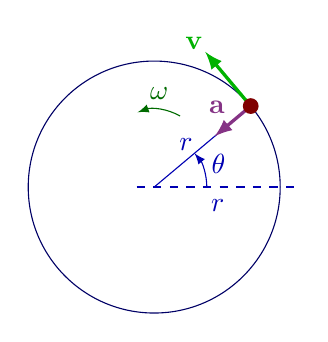
\begin{tikzpicture}
  \def\R{1.6}
  \def\ang{40}
  \coordinate (O) at (0,0);
  \coordinate (X) at (\R,0);
  \coordinate (R) at (\ang:\R);
  \node[inner sep=2] (R') at (R) {};
  \draw[pathcol] (O) circle (\R); %dashed
  \draw[xcol] (O) -- (R) node[midway,below=5,above left=0] {$r$};
  \draw pic[->,"$\theta$",xcol,draw=xcol,angle radius=19,angle eccentricity=1.3] {angle=X--O--R};
  \draw[xcol,dashed] (-0.14*\R,0) -- (1.15*\R,0) node[midway,below=1] {$r$};
  \draw[vector,vcol]
    (R) --++ (\ang+90:0.9) node[above left=-3] {$\vb{v}$};
  \draw[vector,acol]
    (R) --++ (\ang+180:0.6) node[midway,below=0,above left=-1] {$\vb{a}$};
  \fill[red!50!black] (R) circle (0.1);
  \draw[->,omcol] (\ang+30:0.6*\R) arc(\ang+20:\ang+70:0.4*\R) node[midway,above] {$\omega$};
\end{tikzpicture}


% CENTRIPETAL ACCELERATION
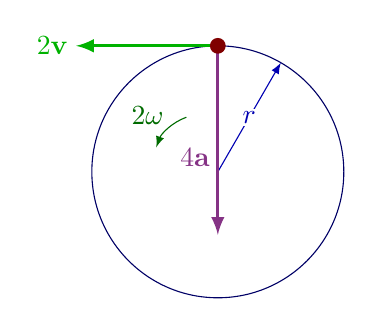
\begin{tikzpicture}
  \def\R{1.6}
  \def\ang{90}
  \coordinate (O) at (0,0);
  \coordinate (R) at (\ang:\R);
  \node[inner sep=2] (R') at (R) {};
  \draw[pathcol] (O) circle (\R); %dashed
  \draw[->,xcol] (O) -- (60:\R) node[midway,fill=white,inner sep=1] {$r$};
  \draw[vector,vcol]
    (R) --++ (\ang+90:1.8) node[left=-1] {$2\vb{v}$};
  \draw[vector,acol]
    (R) --++ (\ang+180:2.4) node[midway,below=0,below left=-1] {$4\vb{a}$};
  \fill[red!50!black] (R) circle (0.1);
  \draw[->,omcol] (\ang+30:0.5*\R) arc(\ang+20:\ang+70:0.4*\R) node[midway,above left=-2] {$2\omega$};
\end{tikzpicture}


% CENTRIPETAL ACCELERATION
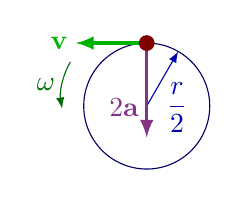
\begin{tikzpicture}
  \def\R{0.8}
  \def\ang{90}
  \coordinate (O) at (0,0);
  \coordinate (R) at (\ang:\R);
  \node[inner sep=2] (R') at (R) {};
  \draw[pathcol] (O) circle (\R); %dashed
  \draw[->,xcol] (O) -- (60:\R) node[midway,below right=-2] {$\dfrac{r}{2}$};
  \draw[vector,vcol]
    (R) --++ (\ang+90:0.9) node[left=-1] {$\vb{v}$};
  \draw[vector,acol]
    (R) --++ (\ang+180:1.2) node[midway,below=0,below left=-1] {$2\vb{a}$};
  \fill[red!50!black] (R) circle (0.1);
  \draw[->,omcol] (\ang+60:1.4*\R) arc(\ang+60:\ang+100:1.1*\R) node[midway,left=-1] {$\omega$};
\end{tikzpicture}


% EARTH
\contourlength{0.7pt}
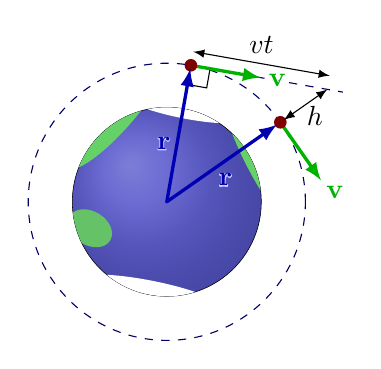
\begin{tikzpicture}
  \def\R{1.76}
  \def\anga{80}
  \def\angb{35}
  \def\E{1.2}
  \coordinate (O) at (0,0);
  \coordinate (A) at (\anga:\R);
  \coordinate (B) at (\angb:\R);
  \coordinate (H) at (\angb:{\R/cos(\anga-\angb)});
  \node[inner sep=1] (A') at (A) {};
  \node[inner sep=1] (B') at (B) {};
  
  % EARTH
  %\draw[dashed,rotate=-11] (0,-1.5*\E) -- (0,1.5*\E);
  \fill[blue!70!black!70] (0,0) circle (1.2);
  \draw[very thin,ball color=blue!70!black!40,fill opacity=0.3] (0,0) circle (\E);
  \begin{scope}[rotate=-11]
    \clip (0,0) circle (\E);
    \fill[white] (0,\E) ellipse ({0.6*\E} and {0.10*\E});
    \fill[white] (0,-\E) ellipse ({0.8*\E} and {0.15*\E});
    \fill[green!70!black!60,rotate=-30] (160:1.1*\E) ellipse ({0.2*\E} and {0.8*\E});
    \fill[green!70!black!60,rotate=40] (-10:1.14*\E) ellipse ({0.2*\E} and {0.9*\E});
    \fill[green!60!black!60,very thick,rotate=-20] % Australia
      (230:0.86*\E) ellipse ({0.25*\E} and {0.18*\E});
    %\draw[dashed] (-\E,0) -- (\E,0);
  \end{scope}
  
  % ORBIT
  \rightAngle{H}{A}{O}{0.35}
  \draw[pathcol,dashed] (O) circle (\R);
  \draw[pathcol,dashed] (A) -- (H) --++ (\anga-90:0.2);
  \draw[<->] (A)++(\anga:0.1*\R) --++ (\anga-90:{\R*tan(\anga-\angb)}) node[midway,above] {$vt$};
  \draw[vector,vcol]
    (A) --++ (\anga-90:0.9) node[scale=1,below=1,right=-1] {\contour{white}{$\vb{v}$}}; %,fill=white,inner sep=0] {$\vb{v}$}; 
  \draw[vector,vcol]
    (B) --++ (\angb-90:0.9) node[scale=1,below right=-2] {$\vb{v}$};
  \fill[red!50!black] (A) circle (0.08);
  \fill[red!50!black] (B) circle (0.08);
  \draw[<->] (H) -- (B') node[midway,below right=-3] {$h$};
  \draw[vector] (O) -- (A') node[midway,below=3,left=-1] {\contour{blue!20}{$\vb{r}$}};
  \draw[vector] (O) -- (B') node[midway,below=6,right=-5] {\contour{blue!20}{$\vb{r}$}};
  
\end{tikzpicture}


% CURVED PATH
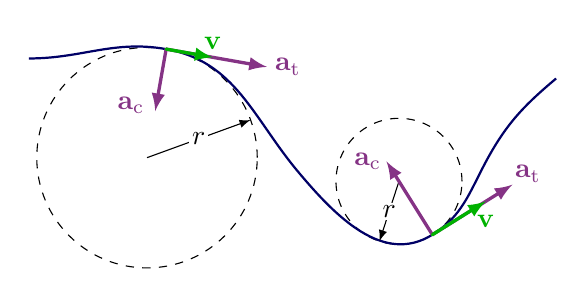
\begin{tikzpicture}
  \def\ul{0.6}
  \def\Ra{1.4}
  \def\Rb{0.8}
  \def\anga{80}
  \def\angb{-58}
  \coordinate (O1) at (0,0);
  \coordinate (O2) at (3.2,-0.3);
  \coordinate (A) at (\anga+60:1.4*\Ra);
  \coordinate (B) at ($(O1)+(\anga:\Ra)$);
  \coordinate (C) at ($(O1)!0.6!(O2)$);
  \coordinate (D) at ($(O2)+(\angb:\Rb)$);
  \coordinate (E) at ($(O2)+(\angb+70:1.4*\Rb)$);
  
  \draw[dashed] (O1) circle (\Ra);
  \draw[dashed] (O2) circle (\Rb);
  \draw[pathcol,thick]
    (A) to[out=0,in=\anga+90]
    (B) to[out=\anga-90,in=130]
    (C) to[out=-50,in=\angb-90]
    (D) to[out=\angb+90,in=\angb-60]
    (E) to[out=\angb+120,in=-140]++ (50:1.4);
  
  % POSITION
  \draw[->] (O1) --++ (\anga-60:\Ra) node[midway,fill=white,inner sep=1] {$r$}; % vector % node[midway,left=5,above right=0] {$\vb{r}$};
  \draw[->] (O2) --++ (\angb-50:\Rb) node[midway,fill=white,inner sep=1] {$r$}; % vector
  
  % ACCELERATION
  \draw[vector,acol]
    (B) --++ (\anga-180:0.8) node[above=2,left=0] {$\vb{a}_\mathrm{c}$};
  \draw[vector,acol]
    (B) --++ (\anga-90:1.3) node[right=-1] {$\vb{a}_\mathrm{t}$};
  \draw[vector,acol]
    (D) --++ (\angb-180:1.1) node[left=-2] {$\vb{a}_\mathrm{c}$}; %above left=-4
  \draw[vector,acol]
    (D) --++ (\angb+90:1.2) node[above right=-3] {$\vb{a}_\mathrm{t}$};
  
  % VELOCITY
  \draw[vector,vcol]
    (B) --++ (\anga-90:0.6) node[above=-1] {$\vb{v}$};
  \draw[vector,vcol]
    (D) --++ (\angb+90:0.8) node[below=1] {$\vb{v}$};
  
\end{tikzpicture}


\end{document}